

Density functional theory (DFT) is a cornerstone of computational physics, widely applied in quantum chemistry, solid state physics, and materials science. It is founded on the Hohenberg-Kohn theorems \cite{hohenberg_inhomogeneous_1964}, which establish that the ground-state properties of a many-electron system are uniquely determined by its electron density.\\
From these insights emerged Kohn-Sham theory\cite{kohn_self-consistent_1965}, which aims to reproduce the ground state density of a complex many-body quantum mechanical system using non-interacting particles governed by the simpler Kohn-Sham equation.
\begin{align}
E_{KS}[\rho ]  = T_S [\rho] + V_{eff}[\rho]
\end{align}
The non-interacting electrons are represented by orbitals $\{\phi_i (\mathbf{r})\}_{i=1,...,n}$, which are pairwise orthogonal and normalized. These combine to form the systems  electron density $\rho(\mathbf{r}) = ||\sum\limits_{i=1}^{N_e} \phi_i(\mathbf{r})||^2$.\\

Despite its remarkable success, KS-DFT has notable limitations. The use of orbitals increases the computational complexity, as the number of functions to be optimized as well as te space on which they live grow with the size of the system. Additionally, its accuracy depends heavily on both the choice of exchange-correlation functional used to approximate many-body effects and the basis set used to define the orbitals.\\


Therefore, there have been many attempts to fulfill the Hohenberg-Kohn promise of a functional dependent solely on electron density. The first orbital-free DFT (OF-DFT) methods relied on empirically guided numerical approximations for the kinetic energy functional \cite{thakkar1992comparison,wang1999orbital} but remained far from chemical accuracy. More recent approaches have employed machine learning to learn the energy functionals of the system. While initial attempts concentrated on toy models \cite{snyder2012finding,li2016pure,meyer2020machine} or focused on single atoms \cite{ghasemi2021artificial}, the field quickly matured to demonstrate stable predictions over different, albeit small, geometries \cite{remme_kineticnet_2023,imoto2021order}. The breakthrough in generalizing to larger systems was achieved with \textsc{M-OFDFT} \cite{zhang_m-ofdft_2023}, which improved upon previous grid-based methods by utilizing atom-centered basis functions and was the first to predict energies with chemical accuracy. However, their gradient descent-based density optimization still fails to converge to the ground state, necessitating unphysical halting criteria. The recent \textsc{Neural SCF} method \cite{song_neuralscf_2024} circumvented these limitations by predicting densities directly but still relies on KS-DFT for energy predictions.
In both cases, prediction quality is limited by the underlying basis set. The employed even-tempered basis sets, produced by algorithms like AutoAux \cite{autoaux}, evenly span the space of electron densities. While these basis sets generalize well and offer arbitrary precision at the cost of increased basis functions, they are not efficient as they aren't optimized for this specific task.
In this work, we introduce differentiable basis integrals, based on the Python library for evaluating basis integrals \textsc{Gbasis} \cite{kim_gbasis_2024}, to optimize basis sets for machine-learned OF-DFT. These optimized basis sets offer improved accuracy in energy and density without increased computational complexity. We explore multiple density fitting algorithms for generating labels for OF-DFT applications and evaluate their effectiveness in training and density optimization of a machine-learned energy functional.
Furthermore, we investigate adaptive basis functions that use a graph neural network to adjust individual atomic basis functions to their local environment. Related work includes Fu et al. \cite{fu_recipe_2024}, who use a graph neural network to directly predict system density through exponents and coefficients but cannot predict energies. For proof of concept, we first apply adaptive basis functions to KS-DFT calculations, following Schütt et al. \cite{schutt_machine_2018}, who used Gaussian processes to predict contraction coefficients for minimal basis sets to accelerate DFT calculations, and Müller et al. \cite{muller_atom--molecule_2023}, who fitted local contraction coefficients to effective atom charges. Our differentiable basis sets enable training an arbitrarily complex neural network to predict both exponents and coefficients, potentially improving KS-DFT calculations with minimal basis sets.
\newpage
\section{Conventions and Notations}
Here we are going to to summarize the conventions that are being followed in this work.
\subsection{Einstein summation}
In this work we are using Einstein summation notation, which is a compact notation for expressing the sum of products of vectors in a vector space. In this notation, summation is implied whenever two indices appear in a product term, one subscript and one superscript. For example, the sum
\begin{align}
    a_i b^i = \sum_{i=1}^n a_i b^i
\end{align}
is implied by the notation. The summation convention is used in this work for all repeated indices, unless otherwise stated.
\subsection{Integral Notation}\label{integral_notation}
We are using Bra-Ket Notation, which is commonly used in quantum mechanics. For two functions $\phi,\psi:\mathbb{R}^3\rightarrow \mathbb{C}$
\begin{align}
    \langle \phi | \psi\rangle &:= \int \phi(\mathbf r)\psi^\dagger(\mathbf r) d\mathbf r
\end{align}
As we are mostly interested in the ground state, which can be described by purely real functions, we can omit the dagger in the notation.
We also note hartree integrals by round brackets, for example
\begin{align}
    (\phi | \psi) &:= \int \int \frac{\phi(\mathbf r)\psi^\dagger(\mathbf r')}{|\mathbf{r}-\mathbf{r'}|} d\mathbf rd\mathbf {r'}
\end{align}
\subsection{Data visualization}\label{boxplots}
To visualize distributions boxplots can give a good overview over the underlying statistics without overcrowding the plotwith to many information. The following visual guide demonstates how the plots used in the work are ment to be interpreted.
\begin{figure}[H]
    \centering
    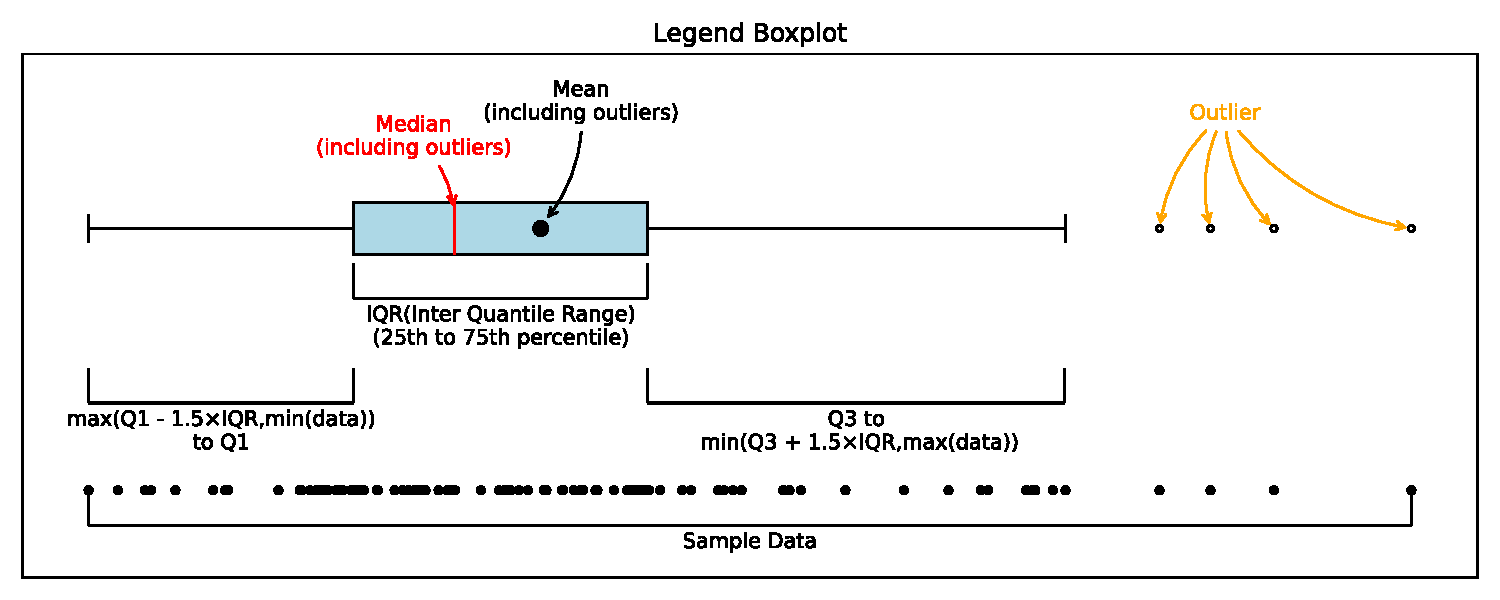
\includegraphics[width=1.\textwidth]{chapters/foundations/images_foundation/legend_boxplot}
    \caption{A boxplot showing the distribution of a toy data set with the important features labeled. Note that the left whiskers is shorted, which indicates that the data is right skewed.}
\end{figure}
Another challenge is the visualisation of the electron density of a molecule. In this work we are
\section{Use of external tools and libraries}
All plots, if not meantioned otherwise, were created by me using the python library matplotlib\cite{hunter_matplotlib_2007}. I used the Large Language models Chatgpt\cite{openai_chatgpt_2024}, Claude\cite{anthropic_claude_2024} and Copilot\cite{github_copilot_2023} for finding references, helping me paraphrase sentences and checking spelling and grammar.